\documentclass{article}

\usepackage[utf8]{inputenc}
\usepackage[german]{babel}
\usepackage{amsmath}
\usepackage{mathtools}
\usepackage{listings}
\usepackage{color}

\lstset{
  language=C,
  numbers=left,
  stepnumber=1,
  numbersep=5pt,
  backgroundcolor=\color[rgb]{0.9,0.9,0.9},
  showspaces=false,
  showstringspaces=false,
  showtabs=false,
  tabsize=2,
  captionpos=b,
  breaklines=true,
  breakatwhitespace=true,
  title=\lstname,
}

\begin{document}

\tableofcontents

\section{Betriebssystem}

\subsection{Definition}

\begin{itemize}
    \item \textbf{Systemsicht} \\
        Alle Programme zur \textbf{Steuerung und Überwachung} von:
        \begin{itemize}
            \item Ausführung v. Benutzerprogrammen
            \item Verteilung der Betriebsmittel
            \item Aufrechterhaltung der Betriebsart
        \end{itemize}
    \item \textbf{Anwendersicht} \\
        \textbf{Virtuelle Maschine}, vereinfachte Ansicht des Computers
\end{itemize}

\subsection{Aufgaben}

\begin{itemize}
    \item \textbf{Hardwareabstraktion}
    \begin{itemize}
        \item einheitliche Sicht auf Geräteklassen
        \item Bibliotheken und Treiber
    \end{itemize}

    \item \textbf{Resourcenverwaltung}
    \begin{itemize}
        \item CPU-Rechenzeit
        \item Speicher
        \item Gerätezugriffe
    \end{itemize}

    \item \textbf{Sicherheitsfeatures}
    \begin{itemize}
        \item Benutzer und Gruppen \textbf{Multi-User}
        \item Parallelbetrieb \textbf{Multitasking}
        \item Schutz for direkten Hardwarezugriffen
    \end{itemize}
\end{itemize}

\subsection{Arten}
\begin{itemize}
    \item \textbf{Mainframe}
        schnelles I/O, viele Prozesse, Transaktionen
    \item \textbf{Server}
        viele Anwender, Netzanbindung    
    \item \textbf{Multiprozessor}
    \item \textbf{Echtzeit}
\end{itemize}

\section{Prozesse}

\subsection{Bestandteile}
\begin{itemize}
    \item eigener Adressraum
    \item Programmcode
    \item Programmdaten
    \item Programm-Counter
    \item Stacks und Stackpointer
    \item Hardwareregister-Inhalte \textit{(Prozess-Kontext)}
    \item Heap-Speicher
    \item Verwaltungsdaten
    \begin{itemize}
        \item Identifier und VaterID
        \item Resourcenliste
        \item Scheduling Parameter
    \end{itemize}
\end{itemize}

\begin{figure}[ht!]
    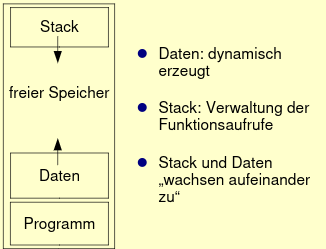
\includegraphics[scale=.75]{pics/processes}
    \caption{Process Control Block PCB}
\end{figure}

\subsection{Hierarchie und Signale}
Jeder Prozess hat \textbf{Vaterprozess} \textit{(Prozesse erzeugen einander)}.

\subsubsection{Fork}
\begin{lstlisting}
    int pid = fork();
    if(pid == 0){
        printf("Ich bin das Kind mit pid=%d\n", getpid());
    }else if(pid > 0){
        printf("Ich bin der Vater, mein Kind hat die pid=%d\n", pid);
    }else{
        printf("Error: fork() war nicht erfolgreich");
    }
\end{lstlisting}

\subsubsection{Signale}
\begin{itemize}
    \item (17) STOP \textit{(Strg-Z oder bg)}
    \item (19) CONT \textit{(fg)}
    \item (15) SIGTERM \textit{(beenden)}
    \item (9) KILL \textit{(abschließen)}
\end{itemize}

\subsection{Prozesserzeugung}
\begin{enumerate}
    \item fork $\rightarrow$ clone $\rightarrow$ do\_fork $\rightarrow$ copy\_process
    \item neue thread\_info in task\_struct
    \item Kind-Status auf TASK\_UNINTERRUPTABLE
    \item copy\_flags
    \item get\_pid: neue PID für Kind
    \item je nach clone-Parametern: kopieren/gemeinsam nutzen
    \item Scheduler
\end{enumerate}

\section{Threads}
\begin{itemize}
    \item Aktivitätsstrang in einem Prozess
    \item gemeinsamer Zugriff auf Daten
\end{itemize}

\subsection{Vergleich: Prozesse/Threads}

\subsubsection{Gemeinsam mit Prozess:}
\begin{itemize}
    \item Adressraum
    \item Programmcode
    \item aktuelle Daten (Variablen/Konstanten)
\end{itemize}

\subsubsection{Separat pro Thread}
\begin{itemize}
    \item PC
    \item SP
    \item Stack
    \item Register
\end{itemize}

\begin{figure}[ht!]
    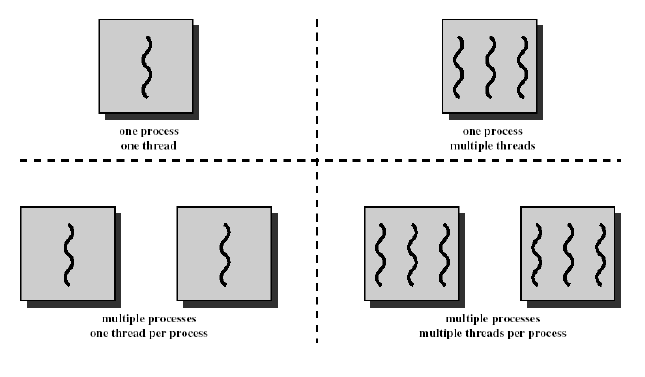
\includegraphics[width=\linewidth]{pics/processes_vs_threads}
    \caption{Unterschied zw. Prozessen und Threads}
\end{figure}

\subsection{User - und Kernel-Level Threads}

\subsubsection{User-Level Threads}
\begin{itemize}
    \item Keine Systemcalls nötig
    \item Blockiert bei I/O
    \item keine Nutzung mehrerer CPUs
    \item Bessere Abstraktion möglich
\end{itemize}

\subsubsection{Kernel-Level Threads}
\begin{itemize}
    \item BS verwalted Threads
    \item Zeitsteuerung nur mit Systemcalls
\end{itemize}

\subsubsection{Kombinierte Threadtypen}
\begin{figure}[ht!]
    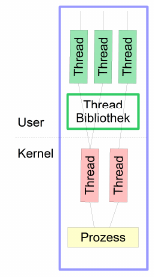
\includegraphics[scale=.8]{pics/ultklt}
    \caption{Komtiniert: ULT, KLT}
\end{figure}

\subsection{Linux Threads und Prozesse}
\textbf{Prozesse} und \textbf{Threads} werden in Linux einheitlich gehandhabt:
\begin{lstlisting}
    // Prozess
    clone(SIGCHLD, 0);
    // Thread
    clone(CLONE_VM | CLONE_FS | CLONE_FILES | CLONE_SIGHAND, 0);
\end{lstlisting}

\begin{figure}[ht!]
    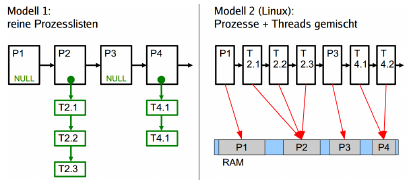
\includegraphics[scale=.8]{pics/linux_ps_th}
    \caption{Linux Prozess- und Threadverwaltung}
\end{figure}


\section{Interrupts}
\subsection{Interrupt-Klassen}
\begin{itemize}
    \item Hardware-Fehler
    \item Timer
    \item I/O
    \item Software-Interrupts
    \begin{itemize}
        \item Arithmetik
        \item Traps
        \item etc.
    \end{itemize}
\end{itemize}

\subsection{Ablauf}
\begin{enumerate}
    \item Interrupt flag wird gesetzt
	\item Nach aktuellem Befehl wird unterbrochen (BS übernimmt Kontrolle)
	\item Prozess-Daten werden gespeichert (wie bei Kontextswitch)
	\item Mittels Interrupt-Vector wird die entsprechende ISR aufgerufen
	\item Diese ist nicht unterbrechbar und so kurz wie möglich
	\item Die ISR ruft dann ein sog. Tasklet auf welches unterbrechbar ist und die eigentliche Arbeit macht
\end{enumerate}

\subsection{Round Robin: I/O- vs CPU-lastig}
\textbf{CPU-lastinge} Prozesse nutzen ihre \textbf{Zeitquanten} vollständig, während \textbf{I/O}
Prozesse \textbf{warten} müssen.

\subsection{Interrupt Handling}
\begin{figure}[ht!]
    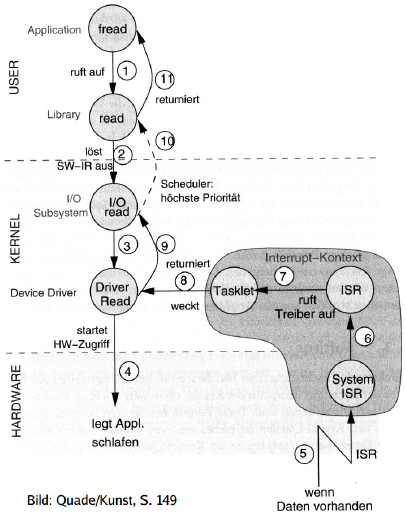
\includegraphics[scale=.8]{pics/isr}
    \caption{Interrupt callgraph}
\end{figure}

\end{document}
